\documentclass[]{article}
\renewcommand{\baselinestretch}{1.25}

\usepackage[margin=1in]{geometry}
\usepackage{physics}
\usepackage{amsmath, amsfonts, amssymb, amsthm}
\usepackage{amssymb}
\usepackage{graphicx}
\usepackage{hyperref}
\usepackage{empheq}
\usepackage{pdfpages}
\usepackage{xcolor}
\usepackage{ulem}

% MATLAB Formatting Code
\usepackage[numbered,framed]{matlab-prettifier}
\lstset{style=Matlab-editor,columns=fullflexible}
\renewcommand{\lstlistingname}{Script}
\newcommand{\scriptname}{\lstlistingname}

% TikZ Things
\usepackage{tikz}
\usetikzlibrary{positioning,shapes}


% Formatting Preferences
\numberwithin{equation}{section}
\usepackage{parskip}
\renewcommand{\figurename}{Fig.}
\allowdisplaybreaks

% Section Heading Settings
\usepackage{enumitem}
\renewcommand{\theenumi}{\alph{enumi}}
\renewcommand*{\thesection}{Problem \arabic{section}}
\renewcommand*{\thesubsection}{\alph{subsection})}
\renewcommand*{\thesubsubsection}{\quad \quad \roman{subsubsection})}

% Math Proof things
\newcommand{\Rel}{\mathcal{R}}
\newcommand{\R}{\mathbb{R}}
\newcommand{\C}{\mathbb{C}}
\newcommand{\N}{\mathbb{N}}
\newcommand{\Z}{\mathbb{Z}}
\newcommand{\Q}{\mathbb{Q}}

\newcommand{\st}{\ : \ }

% Theorem Definition
\newtheorem{definition}{Definition}
\newtheorem{assumption}{Assumption}
\newtheorem{theorem}{Theorem}
\newtheorem{lemma}{Lemma}
\newtheorem{proposition}{Proposition}
\newtheorem{example}{Example}


% Multiagent Robotic Systems Commands
\newcommand{\diam}{\textnormal{diam}}
\newcommand{\radius}{\textnormal{radius}}




%opening
\title{MECH 6V29: Multiagent Robotic Systems- HW 4}
\author{Jonas Wagner}
\date{2022, April 6\textsuperscript{th}}

\begin{document}	

\maketitle

\tableofcontents

%----------------------------------------------------------------------------
\newpage
\section*{Preliminary Notes}

\subsection{Definitions}
\begin{definition} \label{def:graph_def}
	\underline{\emph{Graph}} $G(V,E)$ is constructed with \underline{\emph{vertex set}} \[
		V = \qty{v_1,v_2,\dots,v_n}
	\] of $n$ discrete vertices and \emph{\underline{edge set}} \[
		E = \qty{e_1, \dots, e_m} \subseteq V \cross V
	\] consisting of $m$ edges $e_{k=(i,j)} = (v_i,v_j) \forall_{k=1,\dots,m}$ connecting vertices $v_i$ and $v_j$.
\end{definition}

\begin{definition}\label{def:Delta-disk_graph}
	Let $V = \qty{v_1,v_2,\dots,v_n}$ be vertices.
	\emph{\underline{$\Delta$-Disk Graphs}} are constructed for a particular $\Delta$ such that \[
		(v_i,v_j) \in E \iff \norm{v_i,v_j} \leq \Delta
	\]
\end{definition}

\begin{definition}\label{def:Gabriel_graph}
	Let $V = \qty{v_1,v_2,\dots,v_n}$ be vertices.
	A \emph{\underline{Gabriel Graph}} is defined as $G(V,E)$ in which \[
        \forall_{v_i, v_j \in V} (v_i,v_j) \in E \iff \forall_{v_k \in V} v_k \notin D(v_i,v_j)
    \] where $D(a,b)$ is the closed disc with diameter between $(a,b)$.
    In other words, a disk constructed from two adjacent vertices should not contain any other vertices.
    % \[
	% 	(v_i,v_j) \in E \iff \norm{v_i,v_j} \leq \Delta
	% \]
\end{definition}

\begin{definition} \label{def:graph_properties}
	Let graph $G(V,E)$ with $V = \qty{v_1,\dots,v_n}$ and $E \subseteq V \cross V$.
	\begin{enumerate}
		\item $G(V,E)$ is considered \underline{\emph{undirected}} if\[
			(v_i,v_j) \in E \iff (v_j,v_i) \in E
		\] otherwise, $G(V,E)$ is considered \emph{directed}.
		\item An undirected graph $G(V,E)$ is considered \underline{\emph{connected}} if there exists a path between any two vertices.
		\item A directed graph $G(V,E)$ is considered \underline{\emph{strongly connected}} if there exists a directed path between any two vertices.
		\item A directed graph $G(V,E)$ is considered \underline{\emph{weakly connected}} if the corresponding undirected graph is connected.
	\end{enumerate}
\end{definition}

\begin{definition} \label{def:graph_matrices}
	Let graph $G(V,E)$ with $V = \qty{v_1,\dots,v_n}$ and $E \subseteq V \cross V$.
	\begin{enumerate}
		\item The \underline{\emph{degree matrix}} $\Delta \in \R^{n\cross n}$ is a diagonal matrix defined as \[
			\Delta := \mqty[\dmat{\deg(v_1), \deg(v_2), \ddots, \deg(v_n)}]
		\]
		\item The \emph{\underline{adjacency matrix}} $A \in \R^{n\cross n}$ is a symmetric matrix $(A = A^T)$ defined s.t. \[
			A = [a_{ij}] \st a_{ij} \begin{cases}
				1 &(v_i,v_j) \in V\\
				0 &(v_i,v_j) \notin V
			\end{cases}
		\]
		\item The \emph{\underline{incidence matrix}} $D \in \R^{n \cross m}$ is defined as\[
			D = [d_{ij}] \st d_{ij} \begin{cases}
				1 	&(v_i,-) \in e_{j}\\
				-1	&(-,v_i) \in e_{j}\\
				0	&\text{otherwise}
			\end{cases}
		\]
		\item The \emph{\underline{Laplacian matrix}} $L \in \R^{n \cross n}$ is a symmetric $(L = L^T)$ and strictly semi-positive definite $(L \succeq 0)$ is defined as\[
			L := \Delta - A = D D^T
		\]and\[
			L = \mqty[
				\deg(v_1)	&-a_{12}	&-a_{13}	&\cdots	&-a_{1n}\\
				-a_{21}		&\deg(v_2)	&-a_{23}	&\cdots	&-a_{2n}\\
				\vdots		&\vdots		&\vdots		&\ddots	&\vdots\\
				-a_{n1}		&-a_{n2}	&-a_{n3}	&\cdots	&\deg(v_n)
			]
		\]
		\item For a weighted graph $G(V,E,W)$, the diagonal weighted matrix $W\in \R^{m\cross m}$ is defined as\[
			W = [w_{ij}] \forall_{ij \in E}
		\]
		were $w_{ij}$ are the corresponding weights for $e_{ij} = (v_i,v_j)$.
	\end{enumerate}
\end{definition}



% \begin{definition} \label{def:consensus_dynamics}
% 	Let undirected and unweighted graph $G(V,E)$ with $V = \qty{v_1,\dots,v_n}$ and $E \subseteq V \cross V$.
% 	The \emph{\underline{consensus dynamics}} of network $G(V,E)$ is defined by\[
% 		\forall_{i=1,\dots,n} \ \dot{x}_i = \sum_{j\in \mathcal{N}_i} (x_j - x_i)
% 		\iff \dot{x} = -L x
% 	\] For the case with weighted graph $G(V,E,W)$ with diagonal weight matrix $W = [w_{ij}]$, 
% 	\emph{\underline{weighted consensus dynamics}} are given as\[
% 		\dot{x}_i = \sum_{j\in\mathcal{N}_i} w_{ij} (x_j - x_i) 
% 		\implies \dot{x} = - L_{w} x
% 	\]where weighted Laplacian matrix $L_{w}$ is defined as\[
% 		L_{w} = D W D^T
% 	\]
% \end{definition}


% \begin{definition}\label{def:path_diam_radius_etc}
% 	Let $G(V,E)$ be a undirected graph with $V = \qty{v_1,v_2,\dots,v_n}$ 
% 	and $E = \qty{e_1, \dots, e_m} \subseteq V \cross V$ 
% 	with $e_k = e_{ij} = (v_i, v_j)$.
% 	\begin{enumerate}
% 		\item A \emph{\underline{path}} between two vertices $v_i$ and $v_j$ is a sequence of edges $[e_{i, *}, \dots, e_{*, j}]$ that joins a sequence of vertices $[v_i, \dots, v_j]$.
% 		\item A \emph{\underline{path length}} is the number of edges in the path. 
% 		\item The \emph{\underline{shortest path length}} $l_{i,j}$ is the minimum length of all paths between vertices $v_i$ and $v_j$. 
% 		This quantity is also known as the \emph{\underline{distance}} between $v_i$ and $v_j$, $\text{dist}\qty(v_i,v_j)$.
% 		\item The \emph{\underline{diameter}} of graph $G(V,E)$ is the maximum distance between any two vertices in the graph. 
% 		(i.e.)\[
% 			\diam(G(V,E)) := \max_{v_i,v_j \in V} l_{i,j}
% 		\]
% 		\item The \emph{\underline{eccentricity}} of vertex $v_i$, $l_{i}^{*}$, is the largest distance from $v_i$ to any other vertex in the graph. 
% 		(i.e)\[
% 			l_{i}^{*} := \max_{v_j \in V} l_{i,j}
% 		\]
% 		\item The \emph{\underline{radius}} of graph $G(V,E)$ is the minimum eccentricity of the vertices of the graph.
% 		(i.e)\[
% 			\radius(G(V,E)) := \min_{v_i \in V} l_{i}^{*} = \min_{v_i \in V} \max_{v_j \in V} l_{i,j}
% 		\]
% 	\end{enumerate}
% \end{definition}



% \begin{definition}\label{def:leader_follower_dynamics}
%     Let undirected and unweighted graph $G(V,E)$ with $V = \qty{v_1,\dots,v_n}$ and $E \subseteq V \cross V$.
%     Vertices in $V$ are classified as either \emph{leaders} ($v_i \in V_l$) or \emph{followers} ($v_i \in V_f)$. 
% 	The \emph{\underline{leader-follower}} dynamics of the states within network $G(V,E)$ are defined by\[\begin{cases}
%         \dot{x}_i = - \sum_{j \neq N_i} (x_i - x_j) &\forall_{i \st v_i \in V_{f}}\\
%         \dot{x}_i =  0 &\forall_{i \st v_i \in V_{l}}
%     \end{cases}
% 	\] or equivalently when $V_{l} = \{v_n\}$ (single leader node) \[
%         \dot{x} = \mqty[
%             -L_f & - l\\
%             0 & 0
%         ]
%     \]
% \end{definition}


% --------------- Directed consensus....
% \begin{definition} 
%     Let directed network (di-graph) $G(V,E)$ with $V = \qty{v_1,\dots,v_n}$ and $E \subseteq V \cross V$.
%     \begin{enumerate}
%         \item A directed path ($P : v_i \to v_j$) is a sequence of directed edges constructing a path from $v_i$ to $v_j$.
%         \item 
%     \end{enumerate}
% \end{definition}

% \begin{definition}
%     \textbf{Connectivity of Directed Graphs:} 
%     Let directed network (di-graph) $G(V,E)$ with $V = \qty{v_1,\dots,v_n}$ and $E \subseteq V \cross V$.
%     \begin{enumerate}
%         \item Di-graph $G(V,E)$ is \emph{\underline{strongly connected}} there exists a directed path from any node to every other node.
%         \item Di-graph $G(V,E)$ is \emph{\underline{weakly connected}} the corresponding undirected graph is connected.
%         \item Di-graph $G(V,E)$ is contains a \underline{\emph{rooted out-branching}} if \begin{enumerate}
%             \item $G(V,E)$ does not contain a directed cycle
%             \item $\exists_{v_r \in V}$ such that $\forall_{v_i \neq v_r \in V}$ there is a directed path from $v_r$ to $v_i$.
%         \end{enumerate}
%         \item  Di-graph $G(V,E)$ is considered \underline{\emph{balanced}} if $\deg^{in}(v_k) = \deg^{out}(v_k) \forall_{v_k \in V}$.
%     \end{enumerate}
% \end{definition}

% \begin{theorem}
%     \textbf{Consensus Requirements:}
%     Let directed network (di-graph) $G(V,E)$ with $V = \qty{v_1,\dots,v_n}$ and $E \subseteq V \cross V$
%     \begin{enumerate}
%         \item 
%         \item Di-graph $G(V,E)$ drives to $x$ to $\frac{1}{N} \vb{1} \vb{1}' x(0)$ iff $L$ is balanced and contains a rooted out-branching.
%     \end{enumerate}
% \end{theorem}




% Include Switched Systems & Lyapnov stability....















% \begin{definition} \label{def:tree_graph}
%     A graph $G = (V, E)$ is considered a \emph{\underline{Tree}} if it satisfies any of the following equivalent conditions.
%     \begin{itemize}
%         \item $G$ is connected and acyclic (contains no cycles).
%         \item $G$ is acyclic, and a cycle is formed if any edge is added.
%         \item $G$ is connected, but would be disconnected if any edge is removed.
%         % \item $G$ is connected and $K_3$ is not a minor of $T$.
%         \item Any two vertices in $G$ can be connected by a unique simple path.
%     \end{itemize}
%     If $G$ is a finite graph with $N$ vertices, then these additional conditions are also equivalent:
%     \begin{itemize}
%         \item $G$ is connected and has $N - 1$ edges.
%         % \item G is connected, and every subgraph of G includes at least one vertex with zero or one incident edges. (That is, G is connected and 1-degenerate.)
%         \item $G$ has no simple cycles and has $N-1$ edges.
%     \end{itemize}
% \end{definition}



% Formation Graph & Rigidity -----------------------
\begin{definition} \label{def:form_graph_def}
    Consider a collection of $N$ \underline{\emph{robots}}.
    \emph{\underline{Formation graph}} $G(V, E_f, \omega)$ consists of vertex set \[
        V = \qty{v_1,v_2,\dots,v_N}
    \] of $N$ vertices $v_i$ associated with robot $i$, edge set $E_f$\[
        E_f = \qty{e_1, \dots, e_m} \subseteq V \cross V
    \] of $m$ edges $e_{k=(i,j)} = (v_i,v_j)$ that indicate knowledge of the distance between robots $v_i$ and $v_j$, 
    and $\omega : E_f \to \R_{+}$ which associates a feasible desired inter-agent distance to each pair in $E_f$.
\end{definition}


\begin{definition} \label{def:framework_def}
    Consider a collection of $N$ robots connected in formation graph $G(V, E_f, \omega)$.
    Let each robot be located at \emph{\underline{position}} $P_i \in \R^d$ within euclidean space $(\R^p, \norm{\cdot}_2)$.
    \begin{enumerate}
        \item The \underline{\emph{formation position set}} is defined as the collection of associated robot positions\[
            P = \qty{P_1, \dots, P_N} \subseteq \R^{p \cross p}
        \]
        \item The set of \underline{\emph{pair-wise inter-robot distances}} is defined by \[
            D = \qty{
                d_{ij} \geq 0 \st d_{ij} = d_{ji}, \forall_{i,j \in i, \dots, N}
            }
        \] where $d_{ij}$ is the distance $\norm{P_i - P_j}$.
        \item $D$ is considered \emph{\underline{feasible}} if \[
            \exists_{P_1,\dots,P_N \in \R^d} \st \norm{P_i - P_j} = d_{ij} \forall_{i, j \in \qty{1,\dots,N}}
        \]
        \item A \underline{\emph{framework}} $(G_f, P)$ is a combination of a formation graph $G_f$ and a set of feasible points $P$.
        \item Framework $(G_f, P)$ is considered \emph{\underline{generic}} if $P$ is algebraically independent over $\Q$.
        (i.e. that the points are not collinear in 2-D or co-planer in 3-D)
    \end{enumerate}
\end{definition}

\begin{definition}\label{def:rigid_frame_def}
    Consider frameworks $(G, P_0)$ and $(G, P_1)$.
    \begin{enumerate}
        \item $(G, P_0)$ and $(G, P_1)$ are \emph{\underline{equivalent}} if \[
            \norm{P_0(i) - P_0(j)} = \norm{P_1(i) - P_1(j)} \forall_{(i,j) \in E_f}
        \] meaning $d_{ij}^{(0)} = d_{ij}^{(1)}$ for the vertices that are neighbors.
        \item $(G, P_0)$ and $(G, P_1)$ are \emph{\underline{congruent}} if \[
            \norm{P_0(i) - P_0(j)} = \norm{P_1(i) - P_1(j)} \forall_{(i,j) \in V \cross V}
        \] meaning $d_{ij}^{(0)} = d_{ij}^{(1)}$ for every vertex.
        \item $(G, P_0)$ is \emph{\underline{Globally Rigid}} if \[
            (G, P_1) \ \text{equivalent} \ (G, P_0) \implies (G, P_1) \ \text{congruent} \ (G, P_0)
        \]
        \item $(G, P_0)$ is \emph{\underline{rigid}} if \[
            \exists_{\epsilon>0} \forall_{P_1} \st
            (G, P_1) \ \text{equivalent} \ (G, P_0) 
                \land \forall_{i \in V}  \norm{P_0(i) - P_1(i)} < \epsilon 
            \implies (G, P_1) \ \text{congruent} \ (G, P_1)
        \]
        \textbf{Remark:}
        A framework being rigidity is equivalent to saying that every continuous motion maintaining distances where edges exist also maintains the distances between all other vertex pairs.
    \end{enumerate}
\end{definition}

\begin{definition} \label{def:graph_rigid_test}
    Let $(G, P_0)$ be a $d$-dimensional generic framework.
    \begin{enumerate}
        \item \label{def:rigid_matrix}
            The \emph{\underline{Rigidity Matrix}} is defined by the equations \[
                (x_i - x_j)^T (\dot{x}_i - \dot{x}_j) = 0 \ \forall_{i,j \in E}
            \] resulting in a matrix $R(P_0)$ so that $R(P_0) \dot{P} = 0$.
        \item \label{def:rigid_test}
            \textbf{Rigidity Test:} $(G, P_0)$ is rigid if and only if \[
                \rank(R(P_0)) = \begin{cases}
                    2N - 3 & d=2\\
                    3N - 6 & d=3
                \end{cases}
            \] Additionally, the rank of the rigidity matrix remains the same for all generic realizations, thus $G$ can be called \emph{\underline{Generically Rigid}} if any feasible generic realization is rigid.
    \end{enumerate}
\end{definition}

\begin{definition} \label{def:graph_rigid_min}
    $G_f$ is considered \emph{\underline{minimally rigid}} if it is rigid and the removal of any single edge renders it not rigid.

    Additionally, $G_f$ is minimally rigid if and only if it is rigid and contains \[
        \begin{cases}
            2N - 3 \ \text{edges} & d=2\\
            3N - 6 \ \text{edges} & d=3
        \end{cases}
    \]
\end{definition}

% Problem 1 -------------------------------------------------
\newpage
\section{}
State a summary of \emph{\textbf{Notes 13 - 15}}, (which Include the topics of persistence, combinatorial coverage and graph grammars) preferably by creating a concept map diagram (flow diagram). 
The whole purpose is to make sure that we are clear about the \emph{bigger picture}, and reiterate why are we doing and discussing the specific topics in the class. 
Do not merely write the topics, instead create connections between topics to clarify the flow of information.

\subsection{Big Picture Chart}
% \begin{figure}[h]
% 	\centering
%     \resizebox*{\textwidth}{!}{\begin{tikzpicture}[
% 		empty/.style={coordinate, draw=white!0, fill=white!0, thin, minimum size = 0.1mm},
% 		block/.style={rectangle, draw=blue!80, fill=blue!10, very thick, minimum size = 15mm},
%         subblock/.style={diamond, draw=yellow!80, fill=yellow!10, very thick, minimum size = 15mm, aspect=2.5},
% 		extra/.style={ellipse, draw=red!80, fill=red!10, thick, minimum size = 10mm},
% 		auto,
% 		% roundnode/.style={circle, draw=green!60, fill=green!5, very thick, minimum size=7mm},
% 		% squarednode/.style={rectangle, draw=red!60, fill=red!5, very thick, minimum size=5mm},
% 		]
% 		%Main Nodes
% 		\node[empty]	(center)								{};
		
%         % %Consensus
%         \node[block, text width = 30mm]	(consensus)	[above=2cm of center]	{Consensus Problem $\dot{x}=-L x$};
%         \node[extra]	(con_2)		[above=of consensus]	{Adjacency Matrix: $A$};
%         \node[extra]	(con_1)		[left=of con_2]			{Degree Matrix: $\Delta$};
%         \node[extra]	(con_3)		[right=of con_2]		{Incidence Matrix: $D$};
%         \node[extra]	(con_4)		[above=of con_2]		{Laplacian: $L = \Delta - A = DD^T$};
%         \draw[-]	(consensus.north) 	--	(con_1.south);
%         \draw[-]	(consensus.north) 	--	(con_2.south);
%         \draw[-]	(consensus.north) 	--	(con_3.south);
%         \draw[-]	(con_1.north)		--	(con_4.south);
%         \draw[-]	(con_2.north)		--	(con_4.south);
%         \draw[-]	(con_3.north)		--	(con_4.south);

%         % %Directed Consensus
%         % \node[subblock]	(di_con)	[right=of consensus]	{Directed Consensus};
%         % \draw[-]    (consensus.east) -- (di_con.west);
%         % \node[extra]    (di_con_1)  [right=of di_con]    {Strongly vs Weakly Connected};
%         % \draw[-]    (di_con.east) -- (di_con_1.west);
%         % \node[extra]    (di_con_2)  [below=of di_con_1]    {Rooted Out-branching};
%         % \draw[-]    (di_con.east) -- (di_con_2.west);

%         %Weighted Consensus
%         \node[block, text width = 35mm]	(w_con)	[below=of consensus]	{Weighted Consensus: $\dot{x} = -L_{w} x$};
%         \draw[-]    (consensus.south) -- (w_con);
%         \node[extra, text width = 35mm]    (w_con_2)  [right=of w_con]    {Weighted Laplacian: $L_{w} = D W D^{T}$};
%         \draw[-]    (w_con.east) -- (w_con_2);
%         \node[extra]    (w_con_1)  [above=of w_con_2]    {Weight Matrix: $W$};
%         \draw[-]    (w_con.east) -- (w_con_1);
%         % \node[extra]    (w_con_3)  [below=of w_con_2]    {Static \& Dynamic Weights};
%         % \draw[-]    (w_con.east) -- (w_con_3.west);

%         % %Time-Varying Consensus
%         % \node[subblock]	(tv_con)	[left=of consensus]	{Time Varying Consensus};
%         % \draw[-]    (consensus.west) -- (tv_con.east);
%         % \node[extra]    (tv_con_1) [left=of tv_con] {Switched Networks};
%         % \draw[-]    (tv_con.west) -- (tv_con_1.east);
%         % \node[extra, text width = 40mm]    (tv_con_2) [below=of tv_con_1] {Universal vs Existential Stability};
%         % \draw[-]    (tv_con.west) -- (tv_con_2.east);

%         % %Lyapnov Stability
%         % \node[block]	(lyap)		[left=3cm of center] 	{Lyapnov Stability};
%         % \draw[-]    (lyap.west) -- (tv_con_2.east);
%         % \draw[-]    (lyap.north) -- (consensus.south);

%         % %Leader-Follower System
%         % \node[block]	(lead_follow)		[right=3cm of center] 	{Leader-Follower Network};
%         % \draw[-] (consensus.south) -- (lead_follow.north);

%         %Connectivity Maintenance
%         \node[block]	(cnct_maint)    [below=of w_con] 	{Connectivity Maintenance};
%         \draw[-] (w_con.south) -- (cnct_maint.north);
%         % Ten fun
%         \node[subblock] (ten_fun) [left=of cnct_maint] {Tension Function};
%         \draw[-] (cnct_maint) -- (ten_fun);
%         \node[extra] (ten_fun_1) [left=of ten_fun] {$\mathcal{E} = \sum_{i=1}^{N} \sum_{j=1}^{N} \frac{1}{2} \mathcal{E}_{i,j}(x)$};
%         \draw[-] (ten_fun) -- (ten_fun_1);
%         \node[extra] (ten_fun_2) [above=of ten_fun_1] {$\mathcal{E}_{i,j} = \cfrac{\norm{x_i - x_j}^2}{\Delta - \norm{x_i - x_j}}$};
%         \draw[-] (ten_fun_1) -- (ten_fun_2);
%         \node[extra] (ten_fun_3) [below=of ten_fun_1] {$w_{i,j} = w_{j,i} =  \cfrac{2\Delta - \norm{x_i - x_j}}{\qty(\Delta - \norm{x_i - x_j})^2} > 0$};
%         \draw[-] (ten_fun_1) -- (ten_fun_3);
%         % Hysteresis
%         \node[subblock] (hyst) [right=of cnct_maint] {Hysteresis};
%         \draw[-] (cnct_maint) -- (hyst);
%         \node[extra] (hyst_1) [right=of hyst] {$h_{i,j} = \begin{cases}
%             1 &\norm{x_i - x_j} \leq (\Delta - \epsilon)\\
%             0 &\text{otherwise}
%         \end{cases}$};
%         \draw[-] (hyst) -- (hyst_1);
%         % Consensus eq
%         \node[extra] (cnct_maint_1) [below=of cnct_maint] {$\dot{x}_i = - \sum_{j \in \mathcal{N}_i} h_{i,j} \qty(\cfrac{2\Delta - \norm{x_i - x_j}}{\qty(\Delta - \norm{x_i - x_j})^2}) (x_i - x_j)$};
%         \draw[-] (cnct_maint) -- (cnct_maint_1);
%         \draw[-] (ten_fun_3) -- (cnct_maint_1);
%         \draw[-] (hyst_1) -- (cnct_maint_1);
% 		% %Applications
%         % \node[subblock] (app) [below=2cm of center] {Applications};
%         % % \draw[-] (lead_follow.south) -- (app.north);
%         % % \draw[-] (lyap.south) -- (app.north);
% 		% \node[extra]	(app_2)		[below=of app]	    {Distributed Estimation};
% 		% \node[extra]	(app_1)		[left=of app_2]		{Flocking};
% 		% \node[extra]	(app_3)		[right=of app_2]	{Alignment};
% 		% \draw[-]	(app.south) -- (app_1.north);
% 		% \draw[-]	(app.south) -- (app_2.north);
% 		% \draw[-]	(app.south) -- (app_3.north);




%         % Rigidity

%         % %Main Lines
%         % \draw[-] (applications.west) 	.. controls +(left:5mm) and +(up:3mm)  ..	(ctrl_pblms.north); %controls +(up:5mm) and +(left:5mm)
%         % \draw[-] (applications.east) 	.. controls +(right:5mm) and +(up:3mm) .. (network_model.north);
%         % \draw[-] (ctrl_pblms.south) 	.. controls +(down:7mm) and +(left:7mm)  .. (consensus.west);
%         % \draw[-] (network_model.south)	.. controls +(down:7mm) and +(right:7mm) ..	(consensus.east);





%         % Additional connections
%         \node[empty] (p1) [left=150mm of consensus] {};
%         \draw[-] (consensus) -- (p1);


% 	\end{tikzpicture}}
% 	\caption{Diagram of Course Topics (created w/ TikZ)}
% 	\label{fig:pblm1}
% \end{figure}

\textbf{TO DO:} 
Update all the graph to this time...


% Problem 2 -------------------------------------------------
\newpage
\section{}
% Preliminaries
\subsection*{Preliminaries}
% Persistance ------------------------
\begin{definition}
    
\end{definition}
\begin{definition} \label{def:persistent}
    Consider directed graph $G_F$. 
    \begin{enumerate}
        \item $G_F$ is \emph{\underline{Rigid}} if certain interagent distances are maintained then all interagent distances are maintained when the formation moves smoothly.
        \item $G_F$ is \emph{\underline{Constraint Consistent}} if the directed graph is able to maintain the specified interagent distances.
        \item $G_F$ is considered \emph{\underline{persistent}} if and only if $G_F$ is Rigid and Constraint Consistent.
    \end{enumerate}
\end{definition}



























\newpage
\appendix
\section{MATLAB Code:}\label{apx:matlab}
All code I write in this course can be found on my GitHub repository:\\
\href{https://github.com/jonaswagner2826/MECH6V29_MultiagentRoboticSystems}{https://github.com/jonaswagner2826/MECH6V29\_MultiagentRoboticSystems}

% \bibliographystyle{ieeetran}
% % \bibliography{refs.bib}
% \cite{*}

% 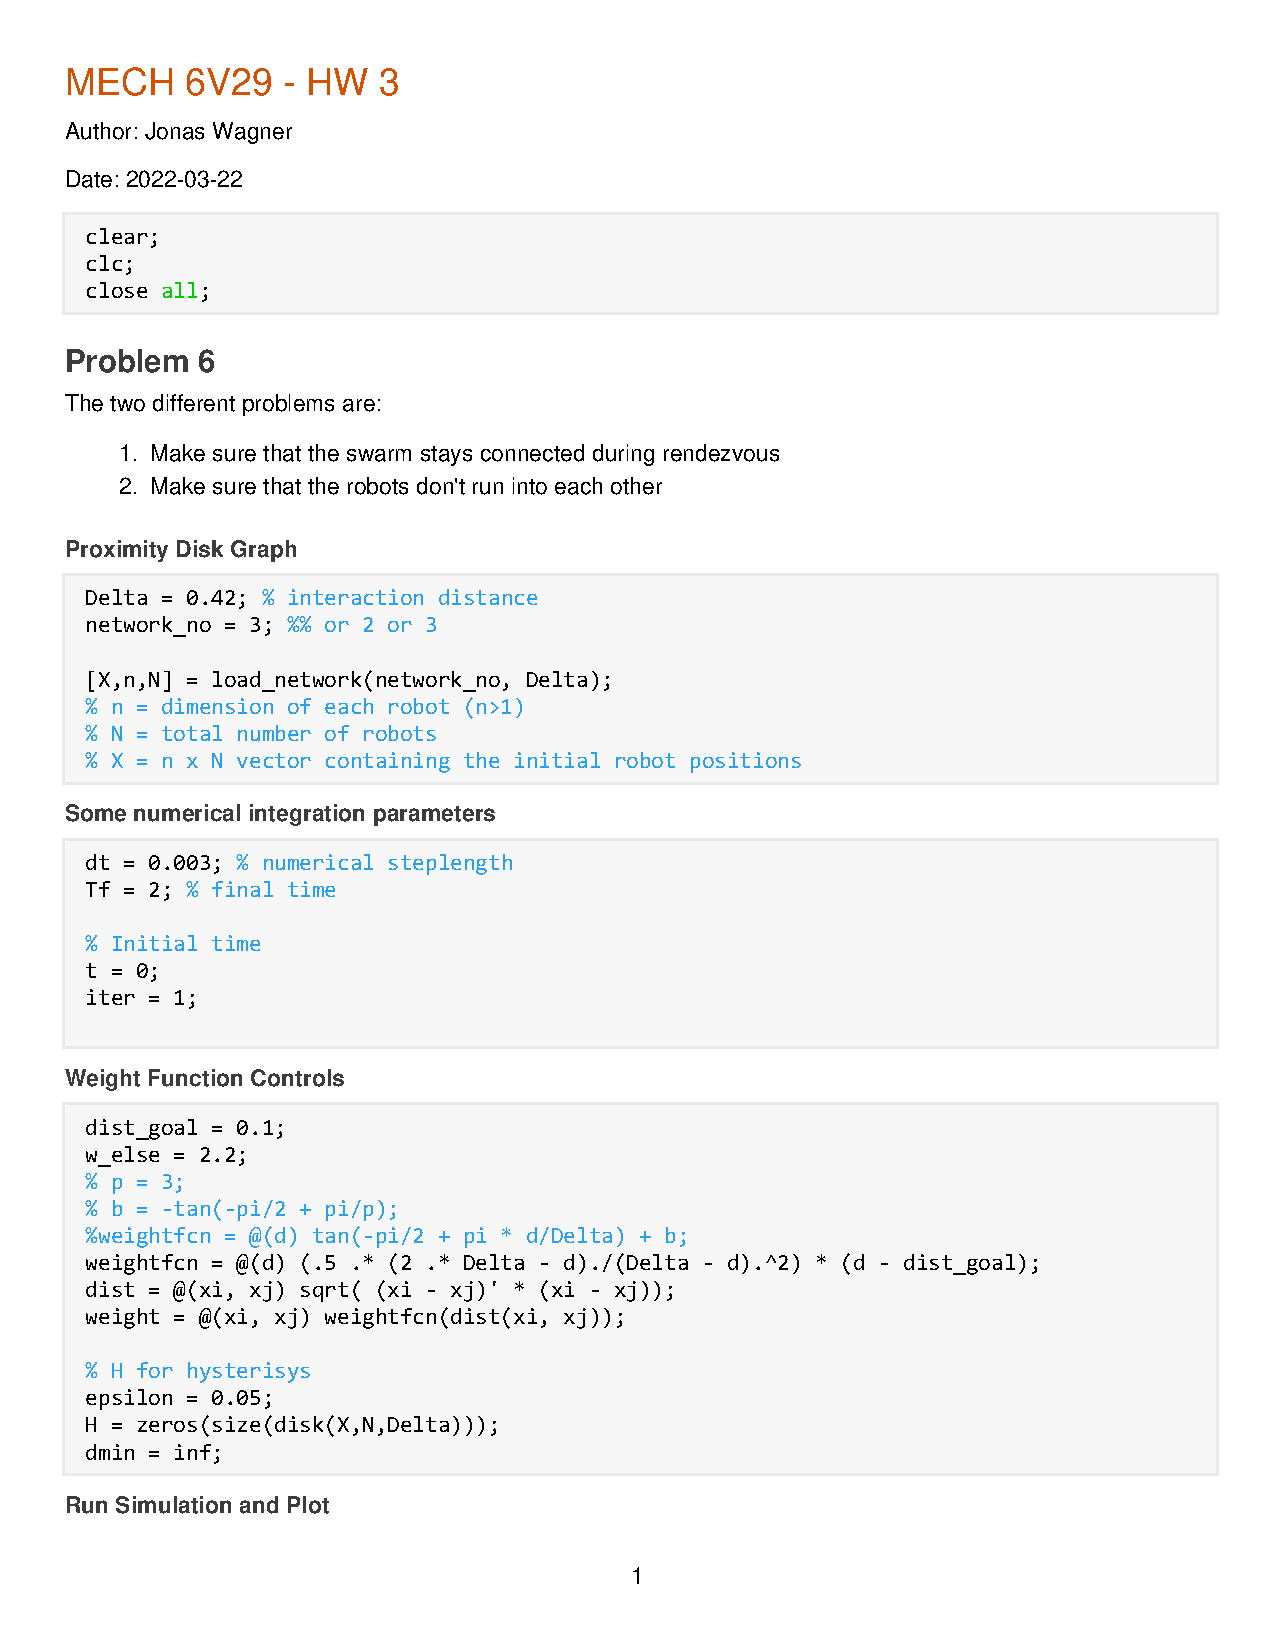
\includepdf[pages=-]{MECH6V29_HW03.pdf}
% 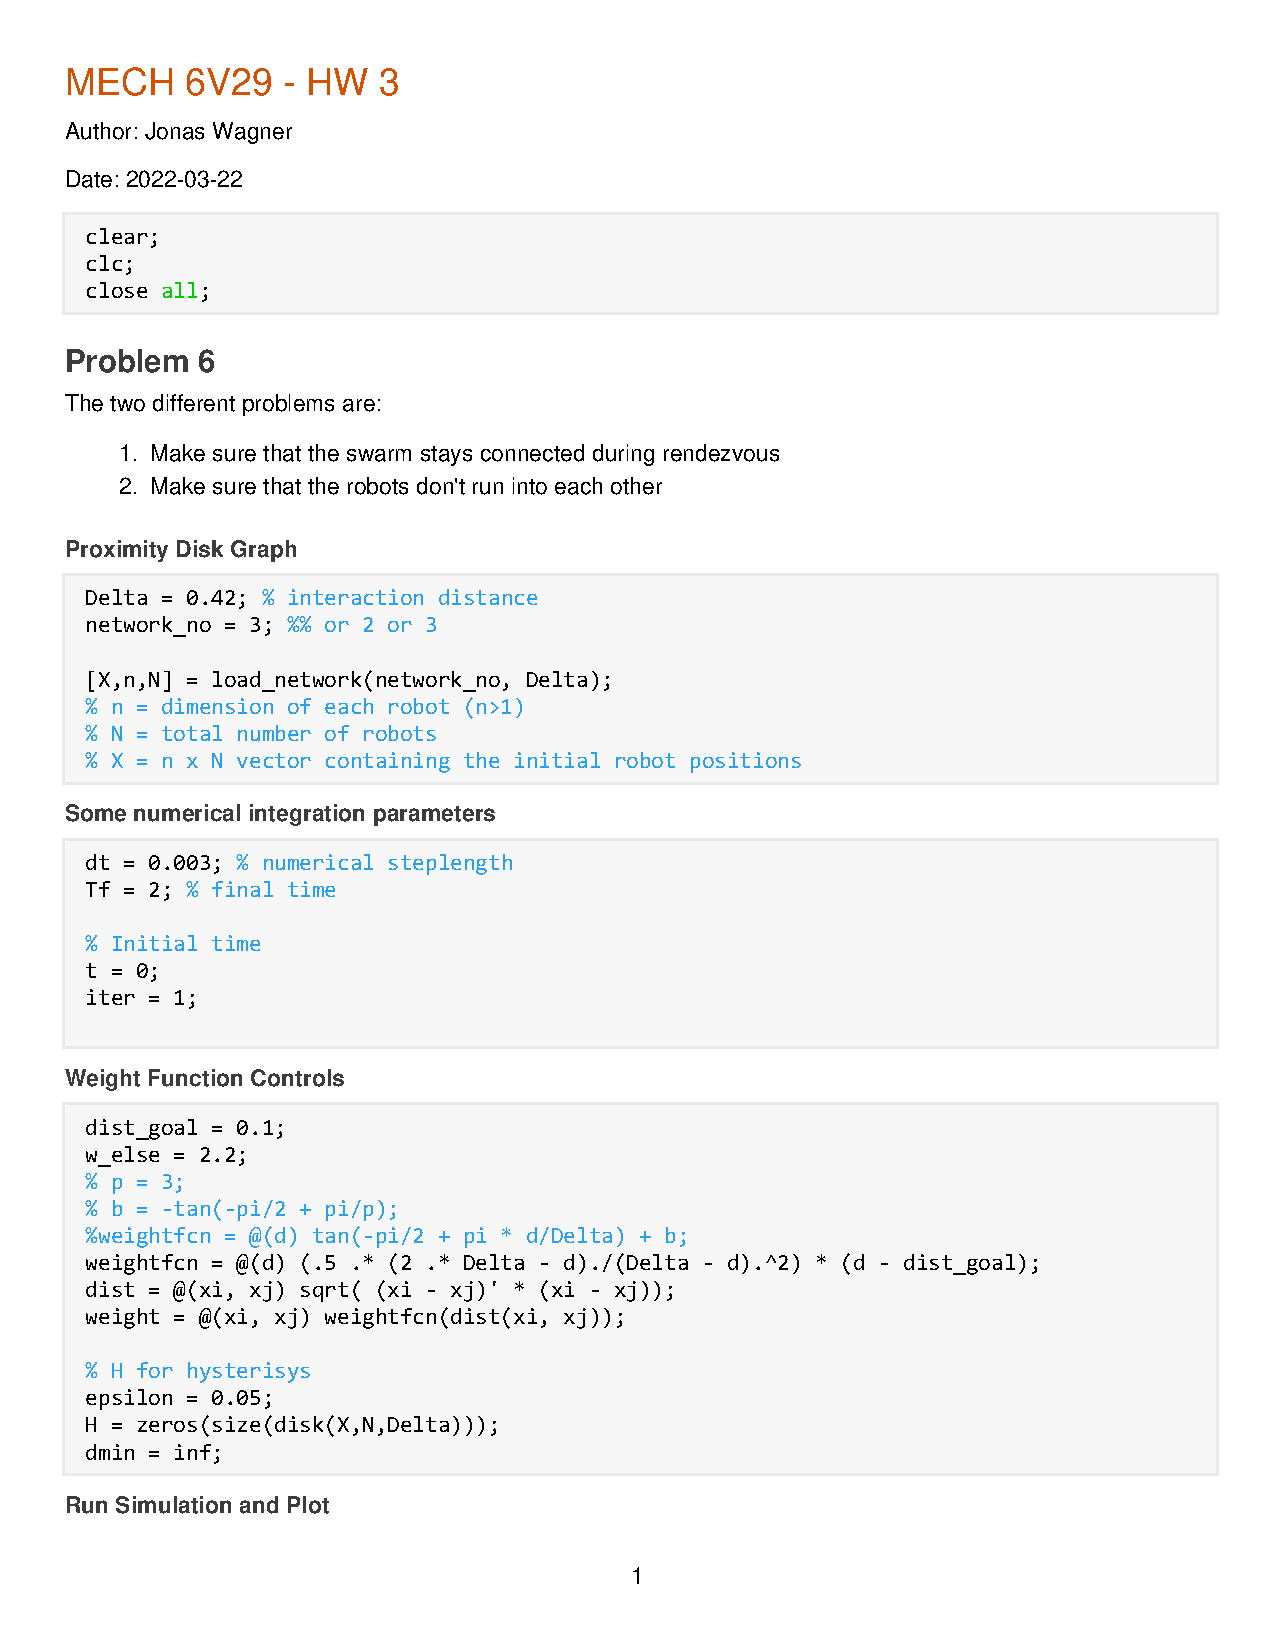
\includepdf[pages=-, nup = 2x2]{MECH6V29_HW03.pdf}


\end{document}
